\section{Q-Learning}
\begin{frame}{}
    \LARGE Reinforcement Learning: \textbf{Q-Learning}
\end{frame}

\begin{frame}[allowframebreaks]{Q-Learning}
    \begin{itemize}
        \item Q-learning is a \textbf{model-free} reinforcement learning algorithm
        \item It \textbf{learns the value of actions in states}, known as the \textbf{Q-value function}
        \item The goal is to find the optimal policy that maximizes the expected cumulative reward
        \item Q-learning is off-policy, meaning it learns the value of the optimal policy independently
        \item It can be used in environments with unknown dynamics, making it suitable for a wide range of problems
    \end{itemize}
\framebreak
    \begin{itemize}
        \item Let $Q$ be an action-value function which hopefully approximates $Q^{\star}$
        \item Q-learning is an algorithm that repeatedly adjusts Q to minimize the Bellman error
        \item Each time we sample consecutive states and actions $(s_t, a_t, s_{t+1}$
    \end{itemize}

    $$Q(s_t,a_t) \leftarrow Q(s_t,a_t) + \alpha \underbrace{\left [ r(s,a) + \gamma \max_{a'} Q(s_{t+1},a') - Q(s_t,a_t) \right ]}_{\text{Bellman Error}}$$
    
\end{frame}

\begin{frame}{Exploration-Exploitation Tradeoff}
\begin{itemize}
    \item Notice: Q-learning only learns about the states and actions it visits.
    \item Exploration-exploitation tradeoff: the agent should sometimes pick suboptimal actions in order to visit new states and actions.
    \item Simple solution: $\epsilon$-greedy policy
    \begin{itemize}
        \item With probability $1 - \epsilon$, choose the optimal action according to Q
        \item With probability $\epsilon$, choose a random action
    \end{itemize}
    \item $\epsilon$-greedy policy still widely used today regardless of simplicity
\end{itemize}
    
\end{frame}

\begin{frame}{Q-Learning Algorithm}
\begin{figure}
\centering
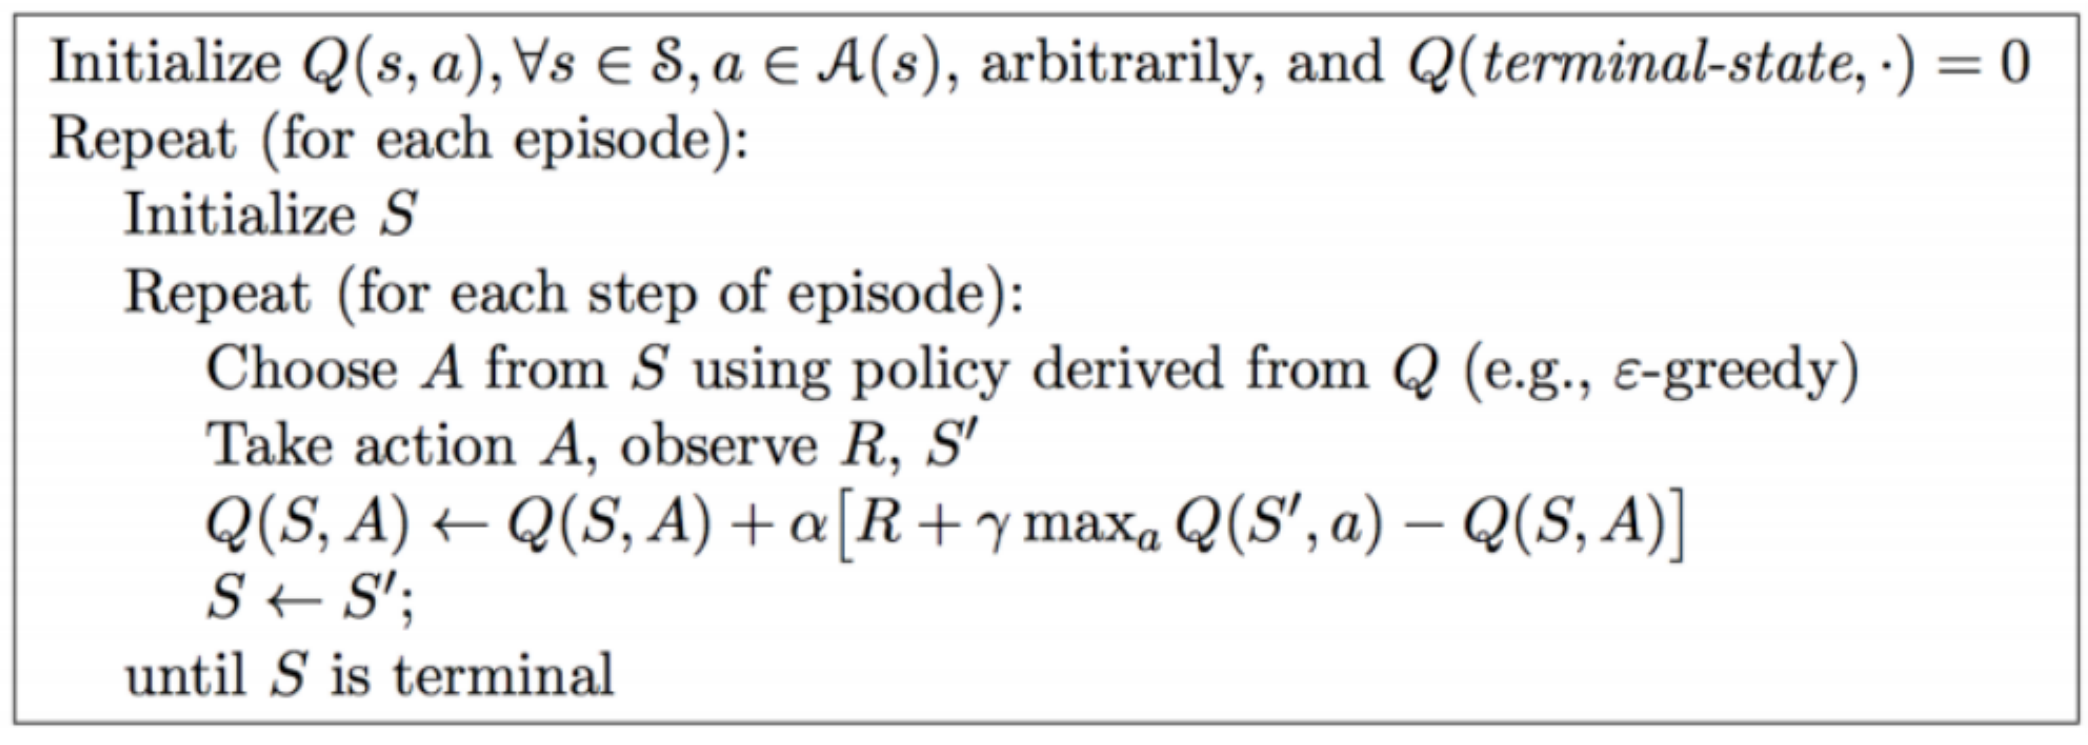
\includegraphics[width=\textwidth,height=0.9\textheight,keepaspectratio]{images/intro/q_learning.png}
\end{figure}
\end{frame}

\begin{frame}{Convergence Properties}
    \begin{itemize}
        \item Q-learning converges to the optimal action-value function $Q^*$ under certain conditions:
        \begin{itemize}
            \item \textbf{Sufficient exploration:} Every state-action pair is visited infinitely often.
            \item \textbf{Learning rate:} The learning rate $\alpha$ decays appropriately, i.e., $\alpha \to 0$ as the number of visits increases, but $\sum_t \alpha_t = \infty$ and $\sum_t \alpha_t^2 < \infty$.
            \item \textbf{Finite MDP:} The environment is a finite Markov Decision Process.
        \end{itemize}
        \item Under these conditions, Q-learning is guaranteed to converge to $Q^*$ with probability 1.
    \end{itemize}
\end{frame}

\begin{frame}{}
\begin{figure}
\centering
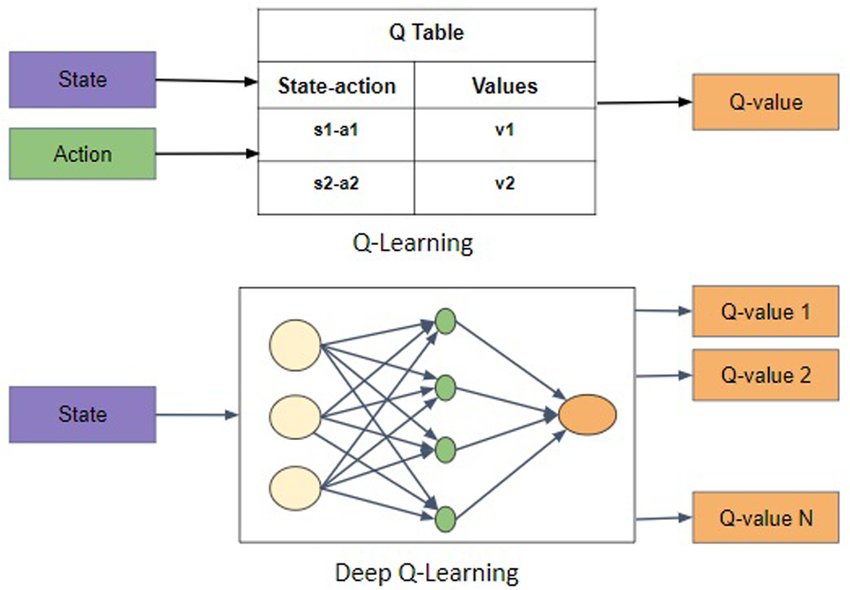
\includegraphics[width=\textwidth,height=0.9\textheight,keepaspectratio]{images/intro/q+deepQ.png}
\end{figure}

\end{frame}